\documentclass[10pt,oneside]{article}
\usepackage[T1]{fontenc}
\usepackage[utf8]{inputenc}
% \usepackage{lmodern}
%\usepackage[adobe-utopia,uppercase=upright,greeklowercase=upright]{mathdesign}
\usepackage[adobe-utopia]{mathdesign}
%\usepackage{minionpro}
% \usepackage{pifont}
% \usepackage{amssymb}
\usepackage{amsmath}
\usepackage[francais]{babel}
% \usepackage[francais]{varioref}
\usepackage[dvips]{graphicx}

\usepackage{framed}
\usepackage[normalem]{ulem}
\usepackage{fancyhdr}
\usepackage{titlesec}
\usepackage{vmargin}
\usepackage{longtable}

\usepackage{ifthen}


%\usepackage{epsfig}
\usepackage{subfig}

\usepackage{multirow}
\usepackage{multicol} % Portions de texte en colonnes
\usepackage{flafter}%floatants après la référence



\usepackage{color}
\usepackage{colortbl}


\definecolor{gris25}{gray}{0.75}
\definecolor{bleu}{RGB}{18,33,98}
\definecolor{bleuf}{RGB}{42,94,171}
\definecolor{bleuc}{RGB}{231,239,247}
\definecolor{rougef}{RGB}{185,18,27}
\definecolor{rougec}{RGB}{255,230,231}
\definecolor{vertf}{RGB}{103,126,82}
\definecolor{vertc}{RGB}{220,255,191}

\newenvironment{rem}[1][\hsize]%
{%
    \def\FrameCommand
    {%
\rotatebox{90}{\textit{\textsf{Remarque}}} 
        {\color{bleuf}\vrule width 3pt}%
        \hspace{0pt}%must no space.
        \fboxsep=\FrameSep\colorbox{bleuc}%
    }%
    \MakeFramed{\hsize#1\advance\hsize-\width\FrameRestore}%
}%
{\endMakeFramed}%


\newenvironment{savoir}[1][\hsize]%
{%
    \def\FrameCommand
    {%
\rotatebox{90}{\textit{\textsf{Savoir}}} 
        {\color{bleuf}\vrule width 3pt}%
        \hspace{0pt}%must no space.
        \fboxsep=\FrameSep\colorbox{bleuc}%
    }%
    \MakeFramed{\hsize#1\advance\hsize-\width\FrameRestore}%
}%
{\endMakeFramed}%


\newenvironment{obj}[1][\hsize]%
{%
    \def\FrameCommand%
    {%
\rotatebox{90}{\textit{\textsf{ $\;$}}} 
        {\color{rougef}\vrule width 3pt}%
        \hspace{0pt}%must no space.
        \fboxsep=\FrameSep\colorbox{rougec}%
    }%
    \MakeFramed{\hsize#1\advance\hsize-\width\FrameRestore}%
}%
{\endMakeFramed}%

\newenvironment{defi}[1][\hsize]%
{%
    \def\FrameCommand%
    {%
\rotatebox{90}{\textit{\textsf{Définition\\}}} 
        {\color{bleuf}\vrule width 3pt}%
        \hspace{0pt}%must no space.
        \fboxsep=\FrameSep\colorbox{bleuc}%
    }%
    \MakeFramed{\hsize#1\advance\hsize-\width\FrameRestore}%
}%
{\endMakeFramed}%

\newenvironment{prop}[1][\hsize]%
{%
    \def\FrameCommand%
    {%
\rotatebox{90}{\textit{\textsf{Propriété\\}}} 
        {\color{bleuf}\vrule width 3pt}%
        \hspace{0pt}%must no space.
        \fboxsep=\FrameSep\colorbox{bleuc}%
    }%
    \MakeFramed{\hsize#1\advance\hsize-\width\FrameRestore}%
}%
{\endMakeFramed}%

\newenvironment{props}[1][\hsize]%
{%
    \def\FrameCommand%
    {%
\rotatebox{90}{\textit{\textsf{Propriétés\\}}} 
        {\color{bleuf}\vrule width 3pt}%
        \hspace{0pt}%must no space.
        \fboxsep=\FrameSep\colorbox{bleuc}%
    }%
    \MakeFramed{\hsize#1\advance\hsize-\width\FrameRestore}%
}%
{\endMakeFramed}%

\newenvironment{exemple}[1][\hsize]%
{%
    \def\FrameCommand%
    {%
\rotatebox{90}{\textit{\textsf{Exemple\\}}} 
        {\color{vertf}\vrule width 3pt}%
        \hspace{0pt}%must no space.
        \fboxsep=\FrameSep\colorbox{vertc}%
    }%
    \MakeFramed{\hsize#1\advance\hsize-\width\FrameRestore}%
}%
{\endMakeFramed}%

\newenvironment{resultat}[1][\hsize]%
{%
    \def\FrameCommand%
    {%
\rotatebox{90}{\textit{\textsf{Résultat\\}}} 
        {\color{rougef}\vrule width 3pt}%
        \hspace{0pt}%must no space.
        \fboxsep=\FrameSep\colorbox{rougec}%
    }%
    \MakeFramed{\hsize#1\advance\hsize-\width\FrameRestore}%
}%
{\endMakeFramed}%

\newenvironment{methode}[1][\hsize]%
{%
    \def\FrameCommand%
    {%
\rotatebox{90}{\textit{\textsf{Méthode\\}}} 
        {\color{rougef}\vrule width 3pt}%
        \hspace{0pt}%must no space.
        \fboxsep=\FrameSep\colorbox{rougec}%
    }%
    \MakeFramed{\hsize#1\advance\hsize-\width\FrameRestore}%
}%
{\endMakeFramed}%

\newenvironment{theo}[1][\hsize]%
{%
    \def\FrameCommand%
    {%
\rotatebox{90}{\textit{\textsf{Théorème\\}}} 
        {\color{rougef}\vrule width 3pt}%
        \hspace{0pt}%must no space.
        \fboxsep=\FrameSep\colorbox{rougec}%
    }%
    \MakeFramed{\hsize#1\advance\hsize-\width\FrameRestore}%
}%
{\endMakeFramed}%

% \usepackage{pstricks}
%\usepackage{minitoc}
% \setcounter{minitocdepth}{4}

\setcounter{tocdepth}{2}

% \mtcselectlanguage{french} 

%\usepackage{draftcopy}% "Brouillon"
% \usepackage{floatflt}
\usepackage{psfrag}
%\usepackage{listings} % Permet d'insérer du code de programmation
\renewcommand{\baselinestretch}{1.2}

% Changer la numérotation des figures :
% ------------------------------------
% \makeatletter
% \renewcommand{\thefigure}{\ifnum \c@section>\z@ \thesection.\fi
%  \@arabic\c@figure}
% \@addtoreset{figure}{section}
% \makeatother
 


%%%%%%%%%%%%
% Définition des vecteurs %
%%%%%%%%%%%%
 \newcommand{\vect}[1]{\overrightarrow{#1}}

%%%%%%%%%%%%
% Définition des torseusr %
%%%%%%%%%%%%

 \newcommand{\torseurcin}[3]{%
\left\{\mathcal{#1} \left(#2/#3 \right) \right\}
}

 \newcommand{\torseurc}[9]{%
\left\{\mathcal{#1}\right\}_{#2}=%
\left\{%
\begin{array}{cc}%
{#3} & {#4}\\%
{#5} & {#6}\\%
{#7} & {#8}\\%
\end{array}%
\right\}_{#9}%
}

% }$$\left\{\mathcal{#1} \right\}_{#2} =%
% \left\{%
% \begin{array}{c}%
%  #3 \\%
%  #4 %
% \end{array}%
% \right\}_{#5}}

%  ------------------------------------------
% | Modification du formatage des sections : | 
%  ------------------------------------------

% Grands titres :
% ---------------

\newcommand{\titre}[1]{%
\begin{center}
      \bigskip
      \rule{\textwidth}{1pt}
      \par\vspace{0.1cm}
      
      \textbf{\large #1}
      \par\rule{\textwidth}{1pt}
    \end{center}
    \bigskip
  }

% Supprime le numéro du chapitre dans la numérotation des sections:
% -----------------------------------------------------------------
\makeatletter
\renewcommand{\thesection}{\@arabic\c@section}
\makeatother


% \titleformat{\chapter}[display]
% {\normalfont\Large\filcenter}
% {}
% {1pc}
% {\titlerule[1pt]
%   \vspace{1pc}%
%   \Huge}[\vspace{1ex}%
% \titlerule]


%%%% Chapitres Comme PY Pechard %%%%%%%%%
% numéro du chapitre
\DeclareFixedFont{\chapnumfont}{OT1}{phv}{b}{n}{80pt}
% pour le mot « Chapitre »
\DeclareFixedFont{\chapchapfont}{OT1}{phv}{m}{it}{40pt}
% pour le titre
\DeclareFixedFont{\chaptitfont}{T1}{phv}{b}{n}{25pt}

\definecolor{gris}{gray}{0.75}
\titleformat{\chapter}[display]%
	{\sffamily}%
	{\filleft\chapchapfont\color{gris}\chaptertitlename\
	\\
	\vspace{12pt}
	\chapnumfont\thechapter}%
	{16pt}%
	{\filleft\chaptitfont}%
	[\vspace{6pt}\titlerule\titlerule\titlerule]

%%%%  Fin Chapitres Comme PY Pechard %%%%%%%%%


% Section, subsection, subsubsection sans serifs :
% % ----------------------------------------------

% \makeatletter
% \renewcommand{\section}{\@startsection{section}{0}{0mm}%
% {\baselineskip}{.3\baselineskip}%
% {\normalfont\sffamily\Large\textbf}}%
% \makeatother

\makeatletter
\renewcommand{\@seccntformat}[1]{{\textcolor{bleu}{\csname
the#1\endcsname}\hspace{0.5em}}}
\makeatother

\makeatletter
\renewcommand{\section}{\@startsection{section}{1}{\z@}%
                       {-4ex \@plus -1ex \@minus -.4ex}%
                       {1ex \@plus.2ex }%
                       {\normalfont\Large\sffamily\bfseries}}%
\makeatother
 
\makeatletter
\renewcommand{\subsection}{\@startsection {subsection}{2}{\z@}
                          {-3ex \@plus -0.1ex \@minus -.4ex}%
                          {0.5ex \@plus.2ex }%
                          {\normalfont\large\sffamily\bfseries}}
\makeatother
 
\makeatletter
\renewcommand{\subsubsection}{\@startsection {subsubsection}{3}{\z@}
                          {-2ex \@plus -0.1ex \@minus -.2ex}%
                          {0.2ex \@plus.2ex }%
                          {\normalfont\large\sffamily\bfseries}}
\makeatother
 
\makeatletter             
\renewcommand{\paragraph}{\@startsection{paragraph}{4}{\z@}%
                                    {-2ex \@plus-.2ex \@minus .2ex}%
                                    {0.1ex}%               
{\normalfont\sffamily\bfseries}}
\makeatother
 
\makeatletter
\renewcommand{\subparagraph}{\@startsection{subparagraph}{5}{\z@}%
                                       {-2ex \@plus-.1ex \@minus .2ex}%
                                       {0.1ex}%
				    {\normalfont\normalsize\sffamily\bfseries}}
\makeatletter
% \makeatletter
% \renewcommand{\subsection}{\@startsection{subsection}{1}{2mm}%
% {\baselineskip}{.3\baselineskip}%
% {\normalfont\sffamily\large\textbf}}%
% \makeatother
% 
% \makeatletter
% \renewcommand{\subsubsection}{\@startsection{subsubsection}{2}{4mm}%
% {\baselineskip}{.15\baselineskip}%
% {\normalfont\sffamily\large\textbf}}%
% \makeatother
% 
% \makeatletter
% \renewcommand{\paragraph}{\@startsection{paragraph}{3}{6mm}%
% {\baselineskip}{.15\baselineskip}%
% {\normalfont\sffamily\large\textbf}}%
% \makeatother
 
\setcounter{secnumdepth}{4}


%  --------
% | Marges |
%  --------


% \setmarginsrb{2.5cm}{1.5cm}{2.5cm}{2cm}{1cm}{1cm}{1cm}{1cm}
\setmarginsrb{1.5cm}{1cm}{1cm}{1.5cm}{1cm}{1cm}{1cm}{1cm}

% Changer les marges localement :
% -----------------------------
\newenvironment{changemargin}[2]{\begin{list}{}{%
\setlength{\topsep}{0pt}%
\setlength{\leftmargin}{0pt}%
\setlength{\rightmargin}{0pt}%
\setlength{\listparindent}{\parindent}%
\setlength{\itemindent}{\parindent}%
\setlength{\parsep}{0pt plus 1pt}%
\addtolength{\leftmargin}{#1}%
\addtolength{\rightmargin}{#2}%
}\item }{\end{list}}



\usepackage{pst-solides3d}
\usepackage{titletoc}
\titlecontents{chapter}[+3pc]
  {\addvspace{10pt}\sffamily\bfseries}
{\contentslabel[{\pscirclebox[fillstyle=solid,fillcolor=gray!25,
linecolor=gray!25,framesep=4pt]{\textcolor{white}{\thecontentslabel}}}]{2.5pc}}
  {}
  {\dotfill \normalfont\thecontentspage\ }

\titlecontents{section}[3pc]
  {\addvspace{2pt}\sffamily}
  {\contentslabel[\thecontentslabel]{1.8pc}}
  {}
  {\dotfill \normalfont\thecontentspage\ }

\titlecontents{subsection}[5pc]
  {\addvspace{2pt}\sffamily}
  {\contentslabel[\thecontentslabel]{1.8pc}}
  {}
  {\dotfill \normalfont\thecontentspage\ }

\titlecontents{subsubsection}[8pc]
  {\addvspace{2pt}\sffamily}
  {\contentslabel[\thecontentslabel]{3pc}}
  {}
  {\dotfill \normalfont\thecontentspage\ }
%{\;\titlerule\;\normalfont\thecontentspage\ }

\titlecontents{paragraph}[9pc]
  {\addvspace{2pt}\sffamily}
  {\contentslabel[\thecontentslabel]{3.5pc}}
  {}
  {\dotfill \normalfont\thecontentspage\ }




\usepackage{style/schemabloc}
%Si le boolen xp est vrai : compilation pour xabi
%Sinon compilation Damien
\newboolean{xp}
\setboolean{xp}{true}

\newboolean{prof}
\setboolean{prof}{true}

\def\xxtitre{\ifthenelse{\boolean{xp}}{
CI 2 -- SLCI : Étude du comportement des Systèmes Linéaires Continus Invariants}{
}}

\def\xxsoustitre{\ifthenelse{\boolean{xp}}{
Chapitre 6 -- Étude des performances des systèmes complexes -- Précision -- Stabilité}{
}}


\def\xxauteur{\ifthenelse{\boolean{xp}}{
\noindent 2013 -- 2014 \\
Xavier \textsc{Pessoles}}{
}}


\def\xxpied{\ifthenelse{\boolean{xp}}{
CI 2 : SLCI -- Cours \\
Ch 6 : Performance des systèmes -- \ifthenelse{\boolean{prof}}{P}{E}%
}{
}}

\usepackage[%
    pdftitle={SLCI - Performance des systèmes},
    pdfauthor={Xavier Pessoles},
    colorlinks=true,
    linkcolor=blue,
    citecolor=magenta]{hyperref}



\usepackage{pifont}
\sloppy
\hyphenpenalty 10000


\begin{document}






% \makeatletter \let\ps@plain\ps@empty \makeatother
%% DEBUT DU DOCUMENT
%% =================




%------------- En tetes et Pieds de Pages ------------


\pagestyle{fancy}
\ifthenelse{\boolean{xp}}{%
\renewcommand{\headrulewidth}{0pt}}{%
\renewcommand{\headrulewidth}{0.2pt}} %pour mettre le trait en haut
%\renewcommand{\headrulewidth}{0.2pt}

\fancyhead{}
\fancyhead[L]{%
\ifthenelse{\boolean{xp}}{%
\noindent\begin{minipage}[c]{2.6cm}%

\includegraphics[width=2cm]{png/logo_ptsi.png}%
\end{minipage}%
}{%
\footnotesize{\textit{\textsf{Lycée François Premier}}}
}}

\ifthenelse{\boolean{xp}}{%
\fancyhead[C]{\rule{12cm}{.5pt}}}{
}


\fancyhead[R]{%
\noindent\begin{minipage}[c]{3cm}
\begin{flushright}
\footnotesize{\textit{\textsf{Sciences Industrielles \\ de l'ingénieur}}}%
\end{flushright}
\end{minipage}
}


\ifthenelse{\boolean{xp}}{%
\fancyhead[C]{\rule{12cm}{.5pt}}}{
}

\renewcommand{\footrulewidth}{0.2pt}

\fancyfoot[C]{\footnotesize{\bfseries \thepage}}
\fancyfoot[L]{%
\begin{minipage}[c]{.2\linewidth}
\noindent\footnotesize{{\xxauteur}}
\end{minipage}
\ifthenelse{\boolean{xp}}{}{%
\begin{minipage}[c]{.15\linewidth}

\includegraphics[width=2cm]{png/logoCC.png}
\end{minipage}}
}


\fancyfoot[R]{\footnotesize{\xxpied}}



\begin{center}
 \huge\textsc{\xxtitre}
\end{center}

\begin{center}
 \LARGE\textsc{\xxsoustitre}
\end{center}

\vspace{.5cm}



\vspace{.5cm}

\begin{center}
\begin{tabular}{ccc}
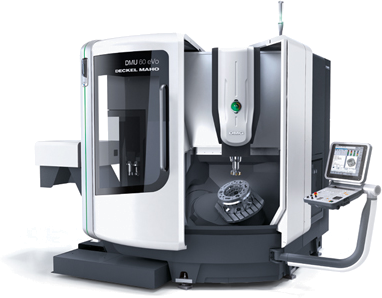
\includegraphics[width=4cm]{png/dmg} &&
%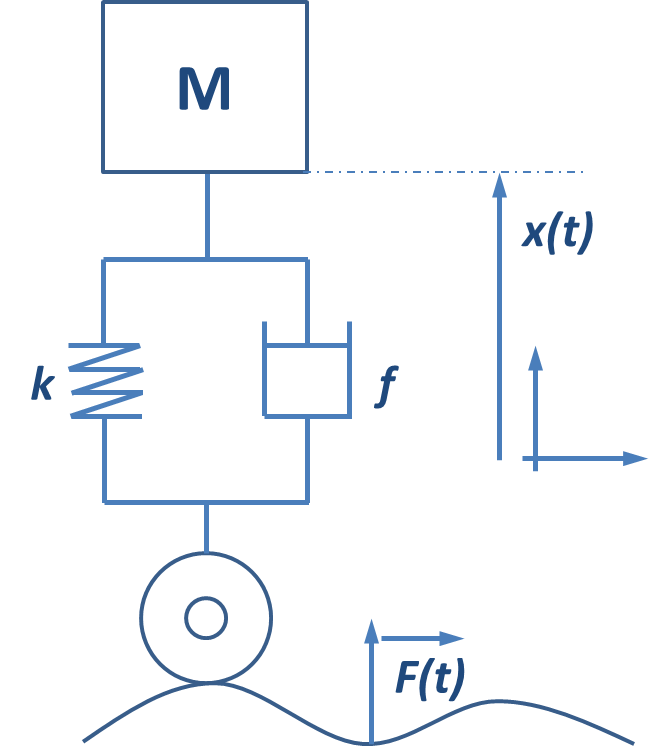
\includegraphics[height=3.5cm]{png/schema} && 
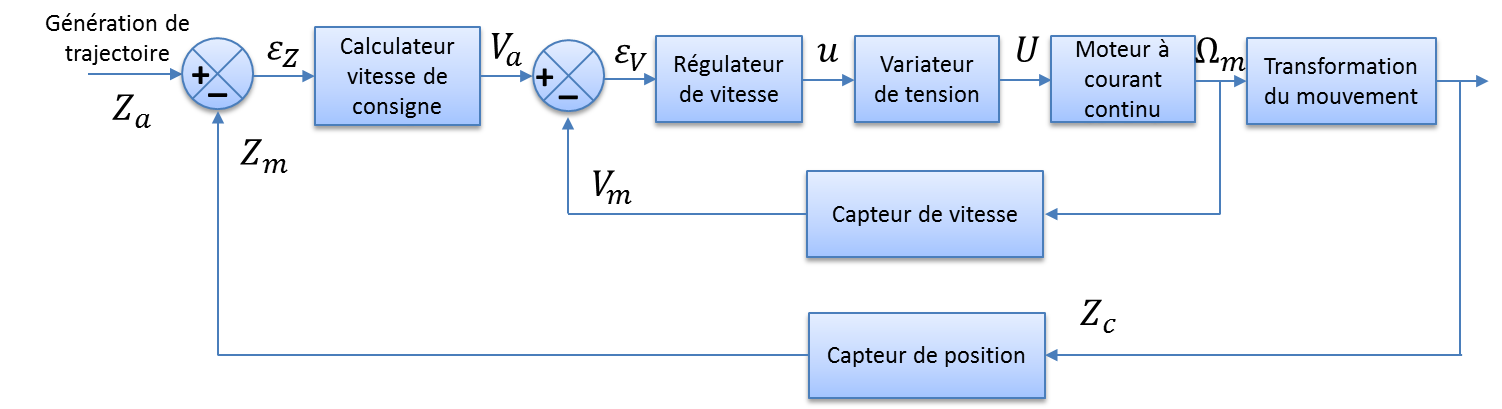
\includegraphics[width=10cm]{png/schemabloc}\\
\textit{DMU 60 eVo Linear} &&
%\textit{Schématisation du mécanisme} &&
\textit{Modélisation par schéma bloc}\\
\textit{Centre d'usinage 5 axes continus\cite{cite1}} && 
\textit{d'un axe numérique asservi \cite{cite2}}\\
\end{tabular}
\end{center}

\vspace{.2cm}

\begin{obj}
\textsc{Problématique :}
\begin{itemize}
\item La modélisation de systèmes multiphysiques donne lieu à des schémas bloc de plus en plus complexes. Comment améliorer la performance de ces systèmes en vue d'améliorer la rapidité, la stabilité ou la précision ?
%\item Comment modéliser un système complexe multiphysique en utilisant la modélisation en schéma bloc et la modélisation dans le domaine de Laplace ?
%\item Comment déterminer la fonction de transfert d'un système dans le but de prévoir son comportement ?
\end{itemize}
\end{obj}

%\begin{savoir}
%\textbf{Savoirs :}
%\begin{itemize}
%\item Mod%-C2.3 : Modèles canoniques du second ordre
%\begin{itemize}
%\item Mod%-C2-S1 : Identifier le comportement d’un système pour l’assimiler à un modèle canonique, à partir d’une réponse temporelle 
%\item Mod%-C2-S2 : Établir un modèle de comportement à partir de relevés expérimentaux
%\item Mod-C2-S3 : On pourra étudier les systèmes du premier ordre présentant un retard pur
%\end{itemize}
%\end{itemize}
%\end{savoir}

\setlength{\parskip}{0ex plus 0.2ex minus 0ex}
 \renewcommand{\contentsname}{}
 \renewcommand{\baselinestretch}{1}

% \vspace{1cm}
\textit{Ce document est en évolution permanente. Merci de signaler toutes
erreurs ou coquilles.}

\tableofcontents

 \renewcommand{\baselinestretch}{1.2}
\setlength{\parskip}{2ex plus 0.5ex minus 0.2ex}

\section{Introduction}


On s'intéresse à un système asservi classique. Les contraintes à respecter vis-à vis du cahier des charges sont des contraintes de stabilité, rapidité et de précision.

\begin{center}
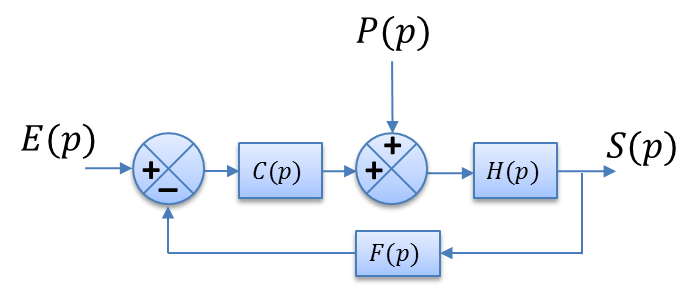
\includegraphics[width=.55\textwidth]{png/bloc1}
\end{center}

\begin{exemple}
Pour modéliser l'axe asservi d'une machine outil la modélisation suivante :
\begin{center}
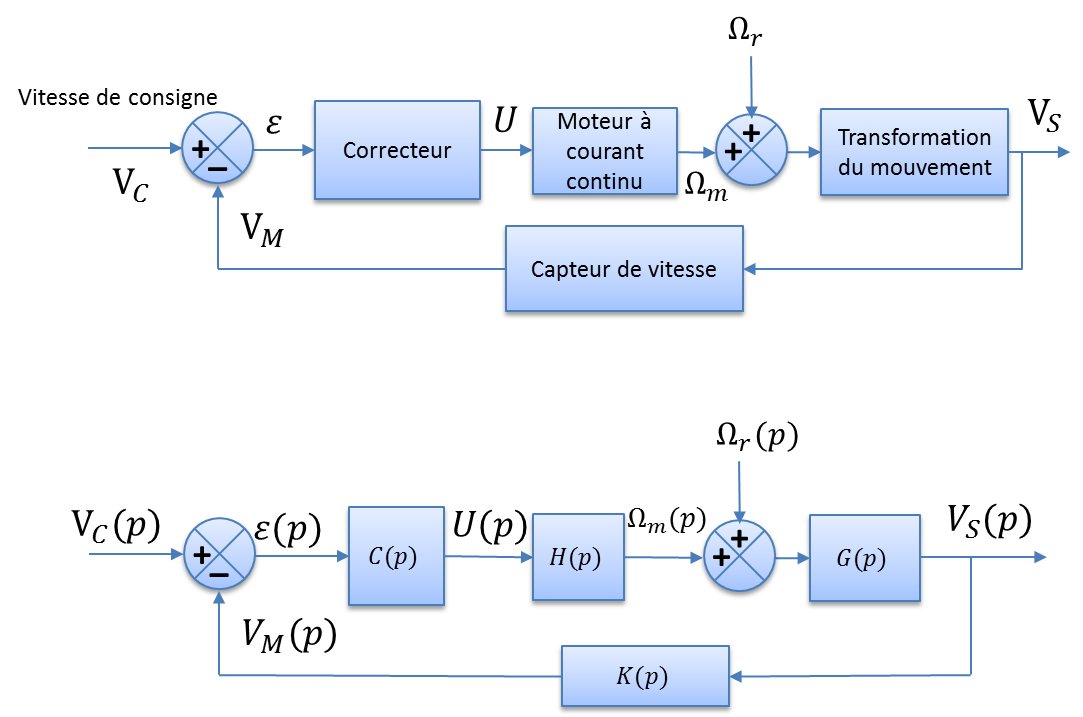
\includegraphics[width=.6\textwidth]{png/bloc2}
\end{center}
On prendra $K(p)=1$, $H(p)$ une fonction de transfert du premier ordre de gain $K_M$ et de constante de temps $\tau$, $G(p)=K_T$ permet de transformer la vitesse de rotation en une vitesse de translation. $C(p)$ est un correcteur de la forme $C(p)=K_C$.
\end{exemple}


\section{Étude du modèle sans perturbation}


\begin{minipage}[c]{.48\linewidth}
\begin{center}
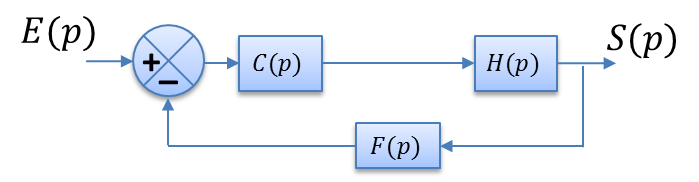
\includegraphics[width=.95\textwidth]{png/bloc11}
\end{center}
\end{minipage}\hfill
\begin{minipage}[c]{.48\linewidth}
Dans ces conditions, exprimons la fonction de transfert en boucle fermée, la fonction de transfert en boucle ouverte et la précision du système :

$$
FTBF(p)
=\dfrac{S(p)}{E(p)}
=\dfrac{C(p)H(p)}{1+C(p)H(p)F(p)}
$$

\end{minipage}


$$
FTBO(p) = C(p) \cdot H(p) \cdot F(p)
$$


Dans tous les cas, $FTBO(p)$ est une fraction rationnelle et peut s'écrire sous la forme suivante : 

$$
FTBO(p)=\dfrac{N(p)}{D(p)}=\dfrac{K\left(1+a_1p +a_2p^2 + ... + a_m p^m \right)}{p^\alpha \left(1+b_1p +b_2p^2 + ... + b_n p^n \right)}
$$


$$
\varepsilon(p)
=\dfrac{1}{1+FTBO(p)} \cdot E(p)
=\dfrac{1}{1+C(p) \cdot H(p) \cdot F(p)} 
$$

\begin{rem}
La précision du système dépend des caractéristiques de la FTBO. On note $K$ son gain et $\alpha$ sa classe.
\end{rem}


Exprimons l'erreur du système :

$$
\lim\limits_{t\to \infty} \varepsilon(t) = \lim\limits_{p\to 0} p \varepsilon(p)
= \lim\limits_{p\to 0} p \dfrac{1}{1+FTBO(p)} \cdot E(p)
= \lim\limits_{p\to 0} p \dfrac{1}{1+\dfrac{K}{p^\alpha}} \cdot E(p)
= \lim\limits_{p\to 0} p \dfrac{p^\alpha}{p^\alpha+K} \cdot E(p)
$$


\begin{exemple}
On considère la perturbation nulle.
\ifthenelse{\boolean{prof}}{%
La fonction de transfert du moteur est de la forme $H(p)=\dfrac{K_M}{1+\tau p}$. 

On a donc :
$$
FTBF(p) = \dfrac{K_C\cdot \dfrac{K_M}{1+\tau p} \cdot K_T}{1+K_C\cdot \dfrac{K_M}{1+\tau p} \cdot K_T}
= \dfrac{K_C K_M K_T}{\left(1+\tau p\right)+K_C K_M K_T}
$$

$$
FTBO(p) = K_C\cdot \dfrac{K_M}{1+\tau p} \cdot K_T
$$


$$
\varepsilon(p)
= \dfrac{1}{1+\dfrac{K_CK_MK_T}{1+\tau p}}\cdot E(p)
= \dfrac{1+\tau p}{1+\tau p+K_CK_MK_T}\cdot E(p)
$$
$$
\varepsilon(p) 
= \dfrac{\dfrac{1}{1+K_CK_MK_T}\left( 1+\tau p\right)}{1+\dfrac{\tau}{1+K_CK_MK_T} p}\cdot E(p)
$$

}{
\rotatebox{90}{
\begin{tabular}{p{5cm}}
\\
\end{tabular}}
}
\end{exemple}

\subsection{Entrée échelon}
Dans ce cas : 
$$
\varepsilon_S =
\lim\limits_{t\to \infty} \varepsilon(t) 
= \lim\limits_{p\to 0} p \dfrac{p^\alpha}{p^\alpha+K} \cdot \dfrac{E_0}{p}
= \lim\limits_{p\to 0}  \dfrac{E_0 p^\alpha}{p^\alpha+K} 
$$

Ainsi :
\begin{itemize}
\item si $\alpha=0$ : $\varepsilon_S = \dfrac{E_0}{1+K}$. Le système est donc plus précis lorsque le gain $K$ de la FTBO augmente;
\item si $\alpha>0$ : $\varepsilon_S = 0$. L'écart statique est donc nul quel que soit $K$.
\end{itemize}

\begin{exemple}
\ifthenelse{\boolean{prof}}{%
$$
\varepsilon_S 
=\lim\limits_{t\to \infty} \varepsilon(t) 
= \lim\limits_{p\to 0} p \varepsilon(p)
= \lim\limits_{p\to 0} p \dfrac{\dfrac{1}{1+K_CK_MK_T}\left( 1+\tau p\right)}{1+\dfrac{\tau}{1+K_CK_MK_T} p}\cdot \dfrac{1}{p}
=\dfrac{1}{1+K_CK_MK_T}
$$

Pour augmenter la précision statique, il faut augmenter le gain du correcteur proportionnel $K_C$.
}{
\rotatebox{90}{
\begin{tabular}{p{4cm}}
\\
\end{tabular}}
}


\end{exemple}


\subsection{Entrée rampe}
Dans ce cas : 
$$
\varepsilon_V =
\lim\limits_{t\to \infty} \varepsilon(t) 
= \lim\limits_{p\to 0} p \dfrac{p^\alpha}{p^\alpha+K} \cdot \dfrac{E_0}{p^2}
= \lim\limits_{p\to 0}  \dfrac{p^\alpha}{p^\alpha+K} \cdot \dfrac{E_0}{p}
$$

Ainsi :
\begin{itemize}
\item si $\alpha=0$ : $\varepsilon_S = \infty$. Le système est donc instable;
\item si $\alpha=1$ : $\varepsilon_S = \dfrac{E_0}{K}$. L'écart de trainage diminue lorsque $K$ augmente;
\item si $\alpha>1$ : $\varepsilon_S = 0$. L'écart de trainage est nul.
\end{itemize}

\begin{exemple}
\ifthenelse{\boolean{prof}}{%
$$
\varepsilon_V
=\lim\limits_{t\to \infty} \varepsilon(t) 
= \lim\limits_{p\to 0} p \varepsilon(p)
= \lim\limits_{p\to 0} p \dfrac{\dfrac{1}{1+K_CK_MK_T}\left( 1+\tau p\right)}{1+\dfrac{\tau}{1+K_CK_MK_T} p}\cdot \dfrac{1}{p^2}
=+\infty
$$

Le système est donc instable lorsqu'il est soumis à une rampe. Utiliser un correcteur intégral de la forme $C(p)=\dfrac{K_C}{p}$ permettrait de stabiliser le système. En augmentant alors $K_C$, on réduirait l'erreur de traînage.

}{
\rotatebox{90}{
\begin{tabular}{p{4cm}}
\\
\end{tabular}}
}


\end{exemple}



\subsection{Entrée en accélération}
Dans ce cas : 
$$
\varepsilon_A =
\lim\limits_{t\to \infty} \varepsilon(t) 
= \lim\limits_{p\to 0} p \dfrac{p^\alpha}{p^\alpha+K} \cdot \dfrac{E_0}{p^3}
= \lim\limits_{p\to 0}  \dfrac{p^\alpha}{p^\alpha+K} \cdot \dfrac{E_0}{p^2}
$$

Ainsi :
\begin{itemize}
\item si $\alpha=0$ : $\varepsilon_A = \infty$. Le système est donc instable;
\item si $\alpha=1$ : $\varepsilon_A = \infty$. Le système est donc instable;
\item si $\alpha=2$ : $\varepsilon_A = \dfrac{E_0}{K}$. L'écart diminue lorsque $K$ augmente.
\end{itemize}

\newpage 

\subsection{Bilan}

\begin{resultat}
La précision d'un système dépend du gain $K$ et de la classe $\alpha$ de la FTBO. 
\begin{center}
\begin{tabular}{|c|c|c|c|c|}
\hline
$e(t)$ & $E(p)$ & $\alpha=0$ & $\alpha=1 $ & $\alpha=2$ \\
\hline
Échelon & $\dfrac{1}{p}$ & $\dfrac{1}{1+K}$ & 0 & 0 \\
\hline
Rampe & $\dfrac{1}{p^2}$ & $\infty$ & $\dfrac{1}{K}$ & 0 \\
\hline
Accélération & $\dfrac{1}{p^3}$ & $\infty$ & $\infty$ & $\dfrac{1}{K}$ \\
\hline
\end{tabular}
\end{center}
\end{resultat}

\begin{rem}
On montre en deuxième année que l'augmentation de $K$ ou de la classe peut être cause d'instabilité.
\end{rem}


\section{Étude du système soumis a une perturbation}
\begin{center}
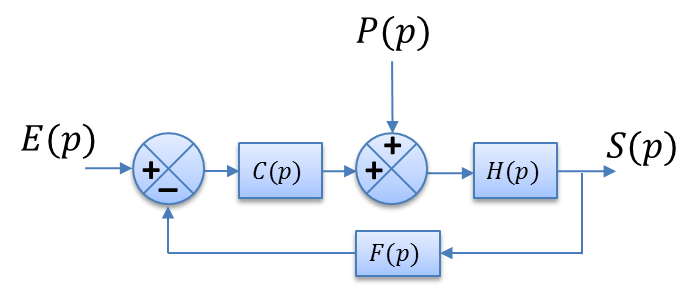
\includegraphics[width=.5\textwidth]{png/bloc1.png}
\end{center}

Exprimons l'erreur du système soumis à perturbation en fonction des deux entrées:
\begin{eqnarray*}
\varepsilon(p) 
&=& E(p)-S(p)\cdot F(p) \\
&=& E(p)-\left(P(p)+\varepsilon(p)C(p)\right)\cdot F(p)H(p) \\
&=& E(p)-P(p)F(p)H(p)-\varepsilon(p)C(p)F(p)H(p) \\
\end{eqnarray*}

\begin{eqnarray*}
\Longleftrightarrow&
\varepsilon(p) \left(1+C(p)F(p)H(p) \right)=E(p)-P(p)F(p)H(p) \\
\Longleftrightarrow&
\varepsilon(p) =\dfrac{E(p)-P(p)F(p)H(p)}{1+C(p)F(p)H(p)}\\
\Longleftrightarrow&
\varepsilon(p) =
\dfrac{1}{1+C(p)F(p)H(p)}E(p)
-\dfrac{F(p)}{1+C(p)F(p)H(p)}P(p)
\end{eqnarray*}

\begin{exemple}
Cas 1 : $C(p)=K_C$

\ifthenelse{\boolean{prof}}{%
$$
\varepsilon(p)=\dfrac{1}{1+G(p)H(p)C(p)}V_c(p) - \dfrac{G(p)}{1+G(p)H(p)C(p)}\Omega_r(p)
$$

$$
\varepsilon(p)=\dfrac{1+\tau p}{1+K_TK_MK_C + \tau p}V_c(p) - K_T
\dfrac{1+\tau_p}{1+K_TK_MK_C + \tau p}\Omega_r(p)
$$

Le système est soumis à une consigne échelon d'amplitude $E_c$ et à une perturbation échelon d'amplitude $E_p$. Dans ce cas, 

$$
\varepsilon(p)=\dfrac{1+\tau p}{1+K_TK_MK_C + \tau p} \dfrac{E_c}{p} - K_T
\dfrac{1+\tau_p}{1+K_TK_MK_C + \tau p} \dfrac{E_p}{p}
$$

$$
\varepsilon_S = \lim\limits_{p\to0} p \varepsilon(p)
=\lim\limits_{p\to0}  \dfrac{1+\tau p}{1+K_TK_MK_C + \tau p} E_c - K_T
\dfrac{1+\tau_p}{1+K_TK_MK_C + \tau p} E_p
$$
$$
\varepsilon_S 
= \dfrac{E_c -  K_T E_p}{1+K_TK_MK_C} 
$$

L'augmentation du gain du correcteur permet de diminuer l'écart statique.

}{
\rotatebox{90}{
\begin{tabular}{p{8cm}}
\\
\end{tabular}}
}
\end{exemple}

\begin{exemple}
Cas 2 : $C(p)=\dfrac{K_C}{p}$


\ifthenelse{\boolean{prof}}{%

}{
\rotatebox{90}{
\begin{tabular}{p{8cm}}
\\
\end{tabular}}
}
\end{exemple}

\section{Étude de la stabilité des systèmes}
Il ne s'agit pas ici de faire une étude exhaustive de la stabilité des systèmes asservis, mais d'avoir une idée sur un des critères de stabilité
\subsection{Système d'ordre 1}
Soit un système du premier ordre sous sa forme canonique :
$$
H(p)=\dfrac{K}{1+\tau p}
$$

Sa réponse temporelle à une entrée échelon d'amplitude $E_0$ est donnée par :
$$
s(t) = E_0 K \left(1-e^{-\dfrac{t}{\tau}}\right)
$$

Le système est instable si $\tau$ est négatif.

\subsection{Système d'ordre 2}
Soit un système du second ordre :
$$
H(p)
=\dfrac{K}{1+\dfrac{2\xi}{\omega_0} p+\dfrac{1}{\omega_0^2} p^2}
=\dfrac{K\omega_0^2}{\omega_0^2+2\xi\omega_0 p+ p^2}
$$


On le sollicite par un échelon d'amplitude $E_0$. En conséquence, $E(p)=\dfrac{E_0}{p}$ et on a :
$$
S(p)=\dfrac{E_0}{p} \cdot \dfrac{K\omega_0^2}{\omega_0^2+2\xi\omega_0 p+ p^2}
$$

\subsubsection{Cas où $\xi>1$}
Dans ce cas, $\omega_0^2+2\xi\omega_0 p+ p^2$ peut se factoriser sous la forme $\left(p-p_1\right)\cdot\left(p-p_2\right)$ avec $p_1 = -\xi\omega_0 + \omega_0 \sqrt{\xi^2-1}$ et $p_2 = -\xi\omega_0 - \omega_0 \sqrt{\xi^2-1}$.

On montre donc que :
$$
S(p)= \dfrac{KE_0}{p} + \dfrac{KE_0 p_2}{p_1-p_2}\cdot \dfrac{1}{p-p_1}
+ \dfrac{KE_0 p_1}{p_2-p_1}\cdot \dfrac{1}{p-p_2}
$$

Et alors, 
$$
s(t) = KE_0\left(1+ \dfrac{ p_2}{p_1-p_2} e^{p_1 \cdot t} + \dfrac{p_1}{p_2-p_1}\cdot e^{p_2 t} \right) \cdot u(t)
$$


Dans ce cas, 

\begin{center}
 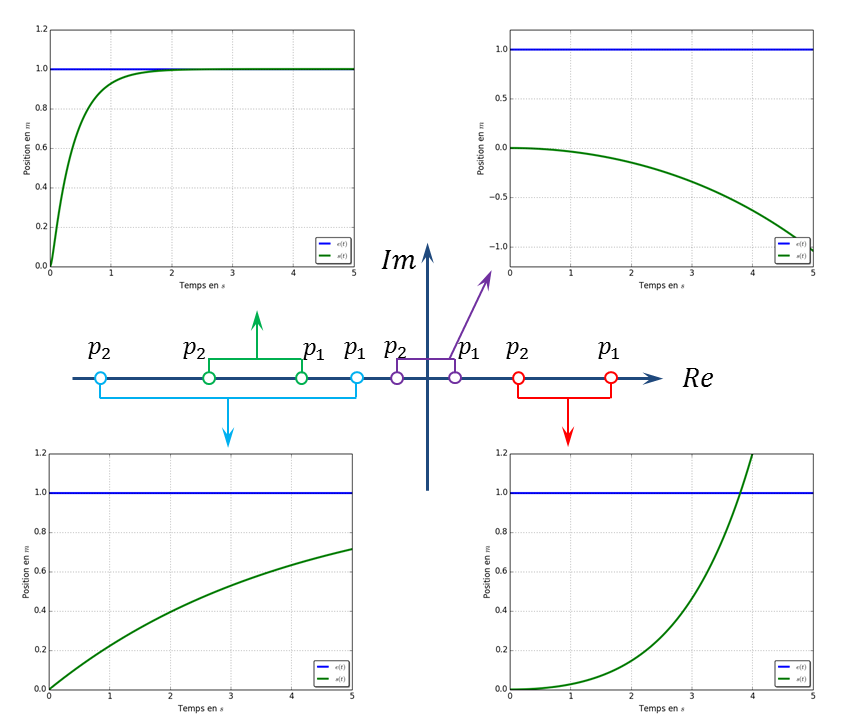
\includegraphics[width=.8\textwidth]{png/poles_1}
\end{center}

\subsubsection{Cas où $\xi=1$}
Dans ce cas, $\omega_0^2+2\xi\omega_0 p+ p^2$ se met sous la forme $\left( p-p_1^2\right) $ avec $p_1 = -\omega_0$.

On montre donc que :
$$
S(p)= \dfrac{KE_0}{p} - \dfrac{KE_0}{p-p_1} - \dfrac{KE_0 \omega_0}{\left(p-p_1\right)^2}
$$

Et alors, 
$$
s(t) = KE_0\left(1- e^{-\omega_0 \cdot t} -\omega_0 t  e^{-\omega_0t} \right) \cdot u(t)
$$

\subsubsection{Cas où $\xi<1$}
Dans ce cas, $\omega_0^2+2\xi\omega_0 p+p^2$ peut se factoriser sous la forme $\left(p-p_1\right)\cdot\left(p-p_2\right)$ avec $p_1 = -\xi\omega_0 + j \omega_0 \sqrt{1-\xi^2}$ et $p_2 = -\xi\omega_0 - j \omega_0 \sqrt{1-\xi^2}$.

On montre donc que :
$$
S(p)= KE_0\left( 
\dfrac{1}{p}
-\dfrac{p+\xi\omega_0}{\left( p+\xi\omega_0\right)^2+\omega_0^2\left(1-\xi^2\right)}
-\dfrac{\xi\omega_0}{\left( p+\xi\omega_0\right)^2+\omega_0^2\left(1-\xi^2\right)}
\right)
$$

Et alors, 
$$
s(t) = KE_0\left(1
- e^{-\xi\omega_0 t}\cdot\cos \left(t\omega_0 \sqrt{1-\xi^2} \right)
- \dfrac{\xi}{\sqrt{1-\xi^2}} e^{-\xi\omega_0 t}\cdot\sin \left(t\omega_0 \sqrt{1-\xi^2} \right)
\right) \cdot u(t)
$$


\begin{center}
 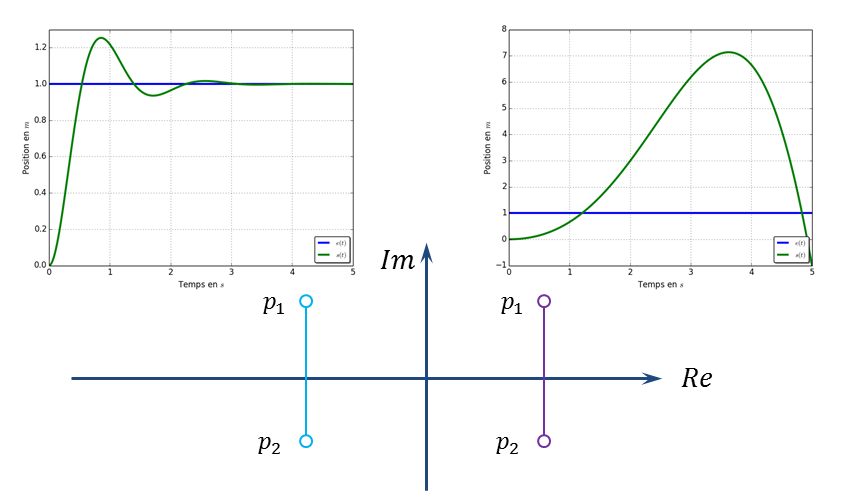
\includegraphics[width=.8\textwidth]{png/poles_3}
\end{center}

%\begin{exemple}
%Cas 3 : $C(p)=K_C$, $C(p)=\dfrac{K_T}{p}$
%\ifthenelse{\boolean{prof}}{
%\rotatebox{90}{
%\begin{tabular}{p{8cm}}
%\\
%\end{tabular}}
%}
%\end{exemple}

\begin{resultat}
On montre qu'un système est stable si les pôles de la \textbf{FTBF} sont à partie réelle \textbf{strictement négative}.
\end{resultat}

\begin{thebibliography}{2}
   \bibitem[1]{cite1} DMU 60 eVo linear, \textit{DMG -- Deckel Maho -- Gildemeiseter}, \url{http://fr.dmg.com}.
   \bibitem[2]{cite2} Programmation des machines-outils à commande numérique (MOCN), \textit{Étienne Lefur et Christophe Sohier}, École Normale Supérieure de Cachan, \url{http://etienne.lefur.free.fr/}.
   \bibitem[3]{cite3} SLCI : Systèmes asservis en boucle fermée : stabilité et précision, \textit{Joël Boiron}, PTSI -- Lycée Gustave Eiffel de Bordeaux.

\end{thebibliography}

\end{document}
